\documentclass{article}

\usepackage[utf8]{inputenc}
\usepackage{ctex}
\usepackage{assignpkg}
\usepackage{xeCJK}
\usepackage{amsmath, amsthm, amssymb}
\usepackage{listings,xcolor}
\usepackage{geometry} % 设置页边距
\usepackage{fontspec}
\usepackage{graphicx}
\usepackage[colorlinks]{hyperref}
\usepackage{setspace}
\usepackage{fancyhdr} % 自定义页眉页脚
\usepackage{enumerate}
\usepackage{ulem}
\usepackage{scalerel}
\usepackage{stackengine}
\usepackage{xcolor}
\usepackage{polynom}
\usepackage{algorithm}
% \usepackage{algorithmic}
\usepackage{algpseudocode}
\usepackage{chngcntr}
\newcommand\showdiv[1]{\overline{\smash{\hstretch{.5}{)}\mkern-3.2mu\hstretch{.5}{)}}#1}}
\newcommand\ph[1]{\textcolor{white}{#1}}

\counterwithin{figure}{subsection}
\counterwithin{table}{subsection}

\newtheorem*{thmm}{定理}
\newtheorem{thm}{定理}[section]
\newtheorem{definition}{定义}[section]
\newtheorem{lemma}{引理}[section]
\newtheorem{corollary}{推论}[section]
\newtheorem{prop}{命题}[section]
\newtheorem{attr}{性质}[section]
\newtheorem*{prf}{证明}
\newtheorem*{lprf}{引理证明}
\newtheorem{exm}{例}[section]
\newtheorem*{sol}{解}


\linespread{1.2}

\definecolor{dkgreen}{rgb}{0,0.6,0}
\definecolor{gray}{rgb}{0.5,0.5,0.5}
\definecolor{mauve}{rgb}{0.58,0,0.82}

\pagestyle{fancy}

\lhead{\CJKfamily{kai} Xi'an JiaoTong University} %以下分别为左中右的页眉和页脚
\chead{}

\rhead{\CJKfamily{kai} 第 \thepage 页}
\lfoot{} 
\cfoot{\thepage}
\rfoot{}
\renewcommand{\headrulewidth}{0.4pt} 
\renewcommand{\footrulewidth}{0.4pt}
%\geometry{left=2.5cm,right=3cm,top=2.5cm,bottom=2.5cm} % 页边距
\geometry{left=3.18cm,right=3.18cm,top=2.54cm,bottom=2.54cm}
\setlength{\columnsep}{30pt}

\renewcommand{\algorithmicrequire}{ \textbf{Input:}} %Use Input in the format of Algorithm
\renewcommand{\algorithmicensure}{ \textbf{Output:}} %UseOutput in the format of Algorithm

\makeatletter

\makeatother

\lstset{
    language    = c++,
    numbers     = left,
    numberstyle={                               % 设置行号格式
        \small
        \color{black}
        % \fontspec{Consolas}
    },
	commentstyle = \color[RGB]{0,128,0}\bfseries, %代码注释的颜色
	keywordstyle={                              % 设置关键字格式
        \color[RGB]{40,40,255}
        % \fontspec{Consolas Bold}
        \bfseries
    },
	stringstyle={                               % 设置字符串格式
        \color[RGB]{128,0,0}
        % \fontspec{Consolas}
        \bfseries
    },
	basicstyle={                                % 设置代码格式
        % \fontspec{Consolas}
        \small\ttfamily
    },
	emphstyle=\color[RGB]{112,64,160},          % 设置强调字格式
    breaklines=true,                            % 设置自动换行
    tabsize     = 4,
    frame       = single,%主题
    columns     = fullflexible,
    rulesepcolor = \color{red!20!green!20!blue!20}, %设置边框的颜色
    showstringspaces = false, %不显示代码字符串中间的空格标记
	escapeinside={\%*}{*)},
}


% \studentIds{计试91 施劲松}{2193512032}
% \studentNames{姓名}{学号}

\assignmentName{复杂网络动力学基础}
\assignmentNumber{1}
\subTitle{}

\date{10/02/2022}

\begin{document}

\makecover

\section{问题 1}

\subsection{问题描述}

在图 \ref{fig:1} 所示的无向网络中,共有 $6$ 个节点 $7$ 条边,$N=6$,$M=7$,试利 用程序求解 $6$ 个节点的介数 $B_i(i=1\ldots 6)$ 和 $7$ 条边的介数 $B_{ij}(e_1\ldots e_7)$,并要求手算 $B_1$ 和 $B_{15}$ 。

\begin{figure}[ht]
    \label{fig:1}
    \centering
    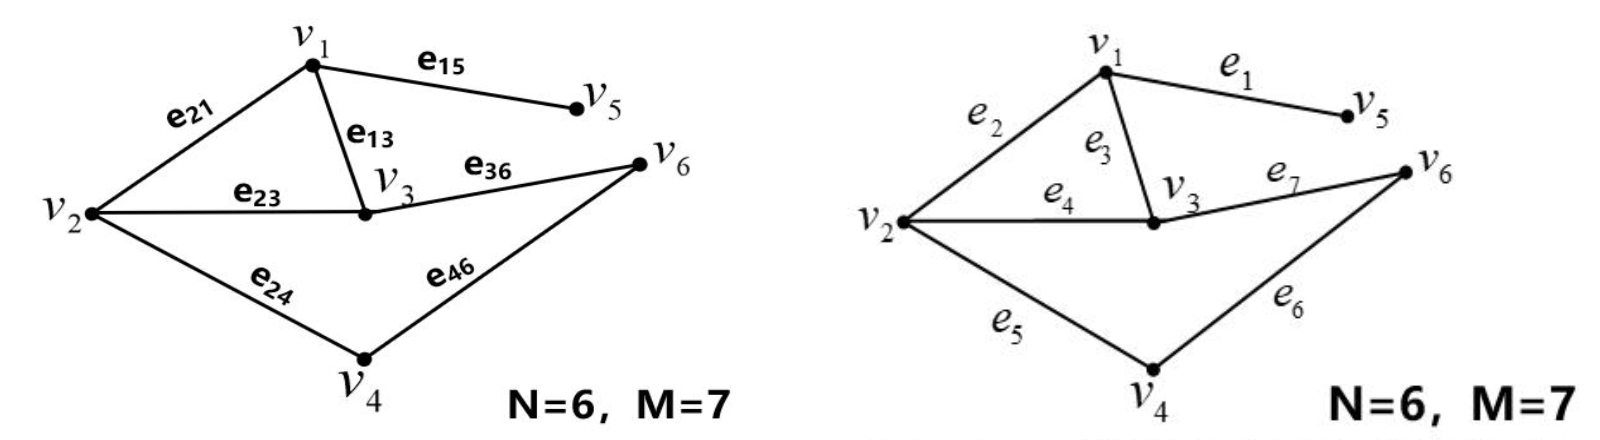
\includegraphics[width=.7\textwidth]{fig1.png}
    \caption{问题 1 无向网络}
\end{figure}

\subsection{实验原理}

节点介数 $B_i$ 表征最短路径途径节点 $v_i$ 的程度。其定义如下:
$$
B_i = \sum_{1\leq j < l \leq N \wedge j\neq i\neq l}\frac{n_{jl}(i)}{n_{jl}}
$$
其中 $n_{jl}$ 为节点 $v_j$ 和 $v_l$ 之间的最短路径条数,$n_{jl}(i)$ 为节点 $v_j$ 和 $v_l$ 之间的最短路径经过节点 $v_i$ 的条数。

同理,边介数 $\tilde{B}_{ij}$ 表征最短路径途径边 $(v_i,v_j)$ 的程度。其定义如下:
$$
\tilde{B}_{ij}=\sum_{1\leq l < m \leq N \wedge (l,m)\neq (i,j)}\frac{N_{lm}(e_{ij})}{N_{lm}}
$$
其中,$N_{lm}$为节点 $v_l$ 与 $v_m$ 之间的最短路径条数;$N_{lm}(e_{ij})$ 为节点 $v_l$ 和 $v_m$ 之间的最短路径且经过边 $e_{ij}$ 的条数。

所以只要求出网络中任意两点之间的最短路径以及对应的最短路径的条数,接着遍历每个点、每条边,就能计算各点及各边的介数。而这用 Floyd 算法就能解决。用 $dp[i][j]$ 表示点 $v_i$ 至 $v_j$ 的最短距离,在转移时多维护一个 $dp\_cnt[i][j]$ 表示最短路径条数即可,时间复杂度:$O(N^3)$。

\subsection{求解过程}

注意到状态转移:
$$
dp[i][j]=
\begin{cases}
    \min_{k=0,1,2,\ldots,n}\{dp[i][k]+dp[k][j]\}, i \neq j\\
    0, i=j
\end{cases}
$$
以及
$$
dp\_cnt[i][j]=
\begin{cases}
    \sum_{dp[i][k]+dp[k][j]=dp[i][j]\wedge k\neq j}dp\_cnt[i][k]\times dp\_cnt[k][j],i\neq j\\
    1,i=j
\end{cases}
$$

故可简单实现如下(\lstinline{C++}):
\begin{lstlisting}
for (int k = 0; k < n; ++k) {
    for (int i = 0; i < n; ++i) {
        for (int j = 0; j < n; ++j) {
            if (i == k || j == k) continue;
            if (dp[i][k] + dp[k][j] < dp[i][j]) {
                dp[i][j] = dp[i][k] + dp[k][j];
                dp_cnt[i][j] = dp_cnt[i][k] * dp_cnt[k][j];
            } else if (dp[i][k] + dp[k][j] == dp[i][j]) {
                dp_cnt[i][j] += dp_cnt[i][k] * dp_cnt[k][j];
            }
        }
    }
}
\end{lstlisting}

手算求解 $B_{1}$ 以及 $\tilde{B}_{15}$ 的过程如下:

\begin{sol}

由无向网络知:
\begin{align*}
    &n_{25}=N_{25}=1\\
    &n_{35}=N_{35}=1\\
    &n_{45}=N_{45}=3\\
    &n_{56}=N_{56}=1
\end{align*}
故:
\begin{align*}
    B_1&=\sum_{i< j}\frac{n_{ij}(1)}{n_{ij}}\\
    &=\frac{n_{25}(1)}{n_{25}}+\frac{n_{35}(1)}{n_{35}}+\frac{n_{45}(1)}{n_{45}}+\frac{n_{56}(1)}{n_{56}}\\
    &=1+1+1+1\\
    &=4
\end{align*}
\begin{align*}
    \tilde{B}_{15}&=\sum_{i< j}\frac{N_{ij}(1)}{N_{ij}}\\
    &=\frac{N_{25}(1)}{N_{25}}+\frac{N_{35}(1)}{N_{35}}+\frac{N_{45}(1)}{N_{45}}+\frac{N_{56}(1)}{N_{56}}\\
    &=1+1+1+1\\
    &=4
\end{align*}

\end{sol}

\subsection{实验数据}

在 \lstinline{bash/zsh} 中输入:
\begin{lstlisting}
$ g++ task_1.cpp -o task_1
$ ./task_1
\end{lstlisting}
再输入该网络:
\begin{lstlisting}
6 7 # 点数、边数

1 5
1 2
1 3
2 3
2 4
4 6
3 6
\end{lstlisting}
得到:
\begin{lstlisting}
node betweenness:
node#1: 4.00
node#2: 2.50
node#3: 2.50
node#4: 0.50
node#5: 0.00
node#6: 0.50
edge betweenness:
edge#1: 4.00
edge#2: 3.00
edge#3: 3.00
edge#4: 1.00
edge#5: 3.00
edge#6: 1.00
edge#7: 3.00
\end{lstlisting}
也即,点 $v_1,v_2,\ldots,v_6$ 的介数分別为:$4,2.5,2.5,0.5,0,0.5$,而边(编号依图 \ref{fig:1}) $e_1,e_2,\ldots,e_7$ 的介数分別为:$4,3,3,1,3,1,3$。

\subsection{实验结果与分析}

实验结果见表 \ref{tab:1} 和表 \ref{tab:2}。

\begin{table}[ht]
    \centering
    \label{tab:1}
    \begin{tabular}{|c|c|c|c|c|c|c|}
        \hline
        结点编号&$1$&$2$&$3$&$4$&$5$&$6$\\
        \hline
        $B_{i}$&$4$&$2.5$&$2.5$&$0.5$&$0$&$0.5$\\
        \hline
    \end{tabular}
    \caption{问题 1 点介数表}
\end{table}


\begin{table}[ht]
    \centering
    \label{tab:2}
    \begin{tabular}{|c|c|c|c|c|c|c|c|}
        \hline
        边编号&$1$&$2$&$3$&$4$&$5$&$6$&$7$\\
        \hline
        $B_{i}$&$4$&$3$&$3$&$1$&$3$&$1$&$3$\\
        \hline
    \end{tabular}
    \caption{问题 1 边介数表}
\end{table}

由上述结果可以得出一些直观性结论:高介数节点通常扮演“枢纽”,往往是图的拓扑中心且会影响 很多节点的连接性;割点往往是高介数节点。高介数边通常扮演“必经之路”,一旦去掉会影响很多节点 的连接性;桥往往是高介数边;而低介数边一旦去掉,影响连通性的概率较小,所以点(边)介数的大小表现了其在网络中的重要性。

\section{问题 2}

\subsection{问题描述}

在互联网的网页链接和搜索引擎中,互联网可以看成一个有向图 \ref{fig:2}(无权有向网络),每一个网页是图的一个节点(顶点),网页间的每一次超链接是图的一个边,Google 公司使用了 PageRank 算法作为搜索引擎的核心算法。下图描述了一个互联网搜索引擎的网页链接关系图,其中有 $7$ 个节点(网页)和 $18$ 条边(超链接),$N=7,M=18$。

基于复杂网络特征向量中心性、Pagerank 算法和书本例 3.6 的学习,试求:
\begin{enumerate}
    \item 网络的邻接矩阵 $\mathrm{B}$、特征向量中心性中最大特征值 $\lambda$ 和所对应的特征向量以及归一化后的特征向量,以及该特征向量中心性的分值;
    \item 网络的 Markov 链的状态转移概率矩阵 $\mathrm{P}$ 及其转置矩阵 $\mathrm{P}^{\mathrm{T}}$,最大特征值 $\lambda_{\mathrm{max}}$,Markov 链的平稳分布,PageRank 值及其直方图,模型参数 $d$ 可选 $0.85$。
\end{enumerate}

\begin{figure}[ht]
    \label{fig:2}
    \centering
    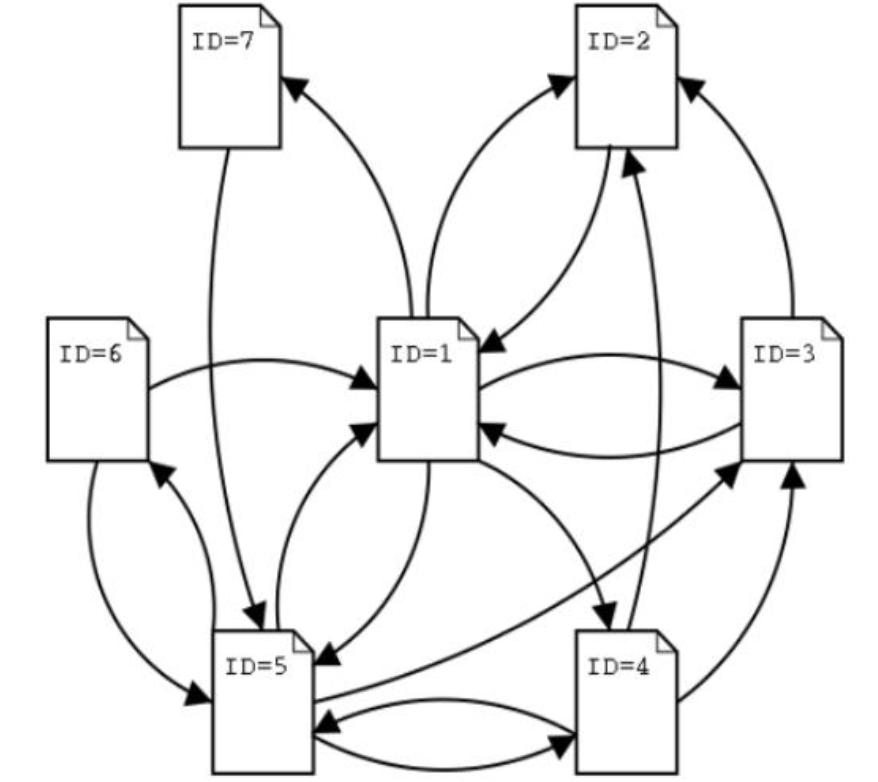
\includegraphics[width=.4\textwidth]{fig2.png}
    \caption{问题 2 有向网络}
\end{figure}

\subsection{实验原理}

矩阵 $\mathrm{B}$ 由网络结构决定:
$$
{\mathrm{B}}_{ij}=
\begin{cases}
    1, (v_i\to v_j)\quad {\text{exists}};\\
    0, (v_i\to v_j)\quad {\text{does\quad not\quad exist}}.
\end{cases}
$$
故由图 \ref{fig:2} 即得:
$$
{\mathrm{B}}=
\begin{pmatrix}
    0&1&1&1&1&0&1\\
    1&0&0&0&0&0&0\\
    1&1&0&0&0&0&0\\
    0&1&1&0&1&0&0\\
    1&0&1&1&0&1&0\\
    1&0&0&0&1&0&0\\
    0&0&0&0&1&0&0\\
\end{pmatrix}
$$

根据定义,满足 $\lambda\vec{x}={\mathrm{B}}\vec{x}$ 的最大特征值 $\lambda_{\mathrm{max}}$ 即为 $\mathrm{B}$ 的特征向量中心性的最大特征值,其对应的归一化后的特征向量的分量即为中心性的分值。而求解特征值即求
$$
\vert {\mathrm{B}} - \lambda{\mathrm{I}}\vert =0
$$
的代数方程。由特征值再求特征向量即求齐次线性方程解。由于高次代数方程极难求解,问题 2 用 \lstinline{python} 来完成。

在互联网的 PageRank 算法中,设网页的浏览行为是 Markov 过程,定义 Markov 链的状态转移概率矩阵为 $\mathrm{P}$。则有:
$$
{\mathrm{P}}_{ij}=\frac{1-d}{N}+d\frac{{\mathrm{B}}_{ij}}{\sum_{l}{\mathrm{B}}_{il}}
$$

而该 Markov 链的平稳分布 $x^{\mathrm{T}}$ 则满足:
$$
{\mathrm{P}^{\mathrm{T}}x}=x
$$
即 $\mathrm{P}^{\mathrm{T}}$ 的最大特征值为 $1$。故要求 2 与要求 1 的求解过程是相仿的,实现时可写成同一函数。

\subsection{求解过程}

由上一节的分析,求解的关键在于如何写一个可求矩阵最大特征值以及对应归一化后的特征向量的函数。借由 \lstinline{python} 中的 \lstinline{numpy} 库,这则可以轻松实现:
\begin{lstlisting}
import numpy as np
# 函数,接收一个矩阵 A,返回最大特征值以及归一化后的特征向量
def get_eigen(A):
    # 获取特征值与特征向量
    eigen_values, eigen_vectors = np.linalg.eig(A)

    i = np.argmax(eigen_values) # 获得最大特征值的索引
    max_eigen_value = eigen_values.max() # 获得最大特征值
    max_eigen_vector = eigen_vectors.T[i] # 获得对应特征向量

    # 最大特征值
    max_eigen_value = np.real(max_eigen_value) # 实化

    # 归一化后的特征向量
    max_eigen_vector = np.real(max_eigen_vector) # 实化
    max_eigen_vector = max_eigen_vector / max_eigen_vector.sum() # 归一化

    # 返回矩阵,最大特征值以及对应归一化后的特征向量
    return A, max_eigen_value, max_eigen_vector.T
\end{lstlisting}

\subsection{实验数据}

由于程序已将邻接矩阵输入,故只需在 \lstinline{bash/zsh} 中输入:
\begin{lstlisting}
$ python3 task_2.py
\end{lstlisting}
得到:
\begin{lstlisting}
邻接矩阵: 
[[0 1 1 1 1 0 1]
[1 0 0 0 0 0 0]
[1 1 0 0 0 0 0]
[0 1 1 0 1 0 0]
[1 0 1 1 0 1 0]
[1 0 0 0 1 0 0]
[0 0 0 0 1 0 0]]
最大特征值: 2.83117721
归一化后的特征向量: 
[[0.22038096]
[0.07784075]
[0.10533488]
[0.14254021]
[0.22038096]
[0.15568150]
[0.07784075]]

状态转移概率矩阵: 
[[0.02142857 0.19142857 0.19142857 0.19142857 0.19142857 0.02142857 0.19142857]
[0.87142857 0.02142857 0.02142857 0.02142857 0.02142857 0.02142857 0.02142857]
[0.44642857 0.44642857 0.02142857 0.02142857 0.02142857 0.02142857 0.02142857]
[0.02142857 0.30476190 0.30476190 0.02142857 0.30476190 0.02142857 0.02142857]
[0.23392857 0.02142857 0.23392857 0.23392857 0.02142857 0.23392857 0.02142857]
[0.44642857 0.02142857 0.02142857 0.02142857 0.44642857 0.02142857 0.02142857]
[0.02142857 0.02142857 0.02142857 0.02142857 0.87142857 0.02142857 0.02142857]]
状态转移概率矩阵的转置: 
[[0.02142857 0.87142857 0.44642857 0.02142857 0.23392857 0.44642857 0.02142857]
[0.19142857 0.02142857 0.44642857 0.30476190 0.02142857 0.02142857 0.02142857]
[0.19142857 0.02142857 0.02142857 0.30476190 0.23392857 0.02142857 0.02142857]
[0.19142857 0.02142857 0.02142857 0.02142857 0.23392857 0.02142857 0.02142857]
[0.19142857 0.02142857 0.02142857 0.30476190 0.02142857 0.44642857 0.87142857]
[0.02142857 0.02142857 0.02142857 0.02142857 0.23392857 0.02142857 0.02142857]
[0.19142857 0.02142857 0.02142857 0.02142857 0.02142857 0.02142857 0.02142857]]
最大特征值: 1.00000000
平稳分布: 
[0.28028780 0.15876449 0.13888182 0.10821960 0.18419813 0.06057067 0.06907750]
\end{lstlisting}

\subsection{实验结果与分析}

由程序运行结果可知:
邻接矩阵 $\mathrm{B}$ 的最大特征值 $\lambda_{\mathrm{max}}$ 为 $2.83117721$,其对应的归一化后的特征向量为:
$$
x^{*}=
\begin{pmatrix}
    0.22038096\\
    0.07784075\\
    0.10533488\\
    0.14254021\\
    0.22038096\\
    0.15568150\\
    0.07784075
\end{pmatrix}
$$
每一维即为特征向量中心性的分值。此处由于是有向图的邻接矩阵,方程 ${\mathrm{B}}\vec{x}=\lambda \vec{x}$ 描述的是链出节点对该点中心性的影响,也就是说,键出的边越多,中心性越大,该点越重要。

而状态转移概率矩阵:
$$
{\mathrm{P}}=
\begin{pmatrix}
    0.02142857&0.19142857&0.19142857&0.19142857&0.19142857&0.02142857&0.19142857\\
    0.87142857&0.02142857&0.02142857&0.02142857&0.02142857&0.02142857&0.02142857\\
    0.44642857&0.44642857&0.02142857&0.02142857&0.02142857&0.02142857&0.02142857\\
    0.02142857&0.30476190&0.30476190&0.02142857&0.30476190&0.02142857&0.02142857\\
    0.23392857&0.02142857&0.23392857&0.23392857&0.02142857&0.23392857&0.02142857\\
    0.44642857&0.02142857&0.02142857&0.02142857&0.44642857&0.02142857&0.02142857\\
    0.02142857&0.02142857&0.02142857&0.02142857&0.87142857&0.02142857&0.02142857
\end{pmatrix}
$$
其转置的最大特征值为 $\lambda_{\mathrm{max}}=1$,对应的归一化后的特征向量(平稳分布的转置):
$$
\vec{x}^{\mathrm{T}}=
\begin{pmatrix}
    0.28028780\\
    0.15876449\\
    0.13888182\\
    0.10821960\\
    0.18419813\\
    0.06057067\\
    0.06907750
\end{pmatrix}
$$

PageRank 能很好地体现一个节的的链入能力,亦即高价值的节点。这与其入度的关系大致为正相关,但若仅考虑入度是较为片面的,因为这会夸大中间“索引”节结的能力。直方图见图 \ref{fig:3},其重要性一目了然,可见 $v_1$ 和 $v_5$ 的 PageRank 值较高,故其重要程度也高,链入能力越强;反之 $v_6$ 和 $v_7$ 则较弱。
\begin{figure}[ht]
    \label{fig:3}
    \centering
    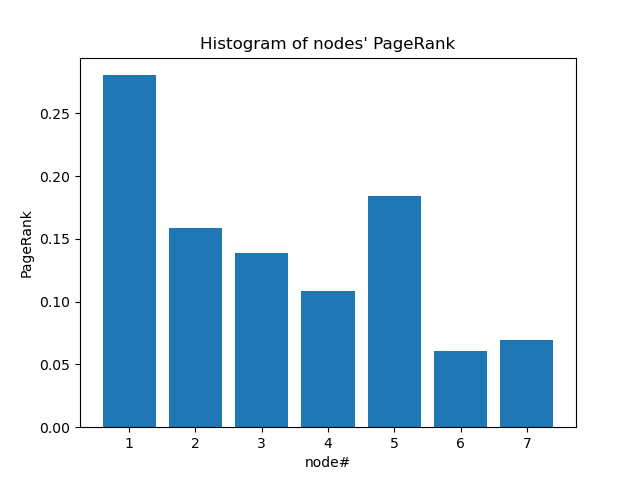
\includegraphics[width=.5\textwidth]{fig3.png}
    \caption{PageRank 直方图}
\end{figure}

\newpage

\section{感想与建议}

复杂网络动力学的学习是网络科学研究中极为重要的一个环节,通过课上课下的学习我对其认知已有一个初步的轮廓,通过本次实验,我更进一步地了解了一些复杂网络中的重要概念与标度,对介数、特征向量中心性以及 PageRank 的作用都有了更深的理解。对今后的学习提供了莫大的帮助。

另外我觉得实验的数据可以加强,实验指导书可以只放一两个简单例子供同学校验。验收可用些强数据,方便检验是否是真正实现了正确的算法,例如用一些随机的种子生成数据是十分方便有效的。

\section{源码}

问题 1 见:\lstinline{./src/task_1.cpp}。

问题 2 见:\lstinline{./src/task_2.py}。

\section{运行}

对于问题 1,请确保安装了 GNU GCC,而后在 \lstinline{bash/zsh} 输入:
\begin{lstlisting}
$ g++ task_1.cpp -o task_1
$ ./task_1
\end{lstlisting}
编译运行,实验数据在源码最下方。若是 Windows 用户,在 \lstinline{cmd} 中输入:
\begin{lstlisting}
> g++ task_1.cpp -o task_1
> .\task_1.exe
\end{lstlisting}

对于问题 2,请确保安装了 \lstinline{python3} 以及依赖包 \lstinline{numpy}(可使用 conda 或 pip 安装),conda 安装命令并运行方法:
\begin{lstlisting}
$ conda create -n lab1 numpy
$ conda activate lab1
$ python3 task_2.py
\end{lstlisting}

另外,源码采用 utf-8 编码,若开启编辑器中文乱码,请切换至 utf-8 编码重新打开。

\end{document}